\documentclass[aspectratio=169,11pt]{beamer}

\usetheme{Madrid}
\usecolortheme{default}
\setbeamertemplate{navigation symbols}{}
\setbeamertemplate{footline}[frame number]
\setbeamerfont{title}{size=\large}
\setbeamerfont{frametitle}{size=\large}

\usepackage{booktabs}
\usepackage{amsmath,amssymb}
\usepackage{graphicx}
\usepackage{tikz}
\usetikzlibrary{arrows.meta,positioning}

\title{Transformixer:Attention-Based Variate Mixing\\without Positional Bias for Multivariate Forecasting}
\author{Morteza Ziabakhsh\\University of Tehran}
\date{}

\begin{document}

%---------------------------------------------------------------------
\begin{frame}
  \titlepage
\end{frame}

%---------------------------------------------------------------------
\begin{frame}{Outline}
  \begin{enumerate}
    \item Motivation and problem
    \item Background: xLSTM-Mixer
    \item Proposed model: Transformixer
    \item Why Transformer mixing (beyond equivariance)
    \item Experimental setup
    \item Main results
    \item Mixer ablation
    \item Permutation \& attention analysis
    \item Training throughput
    \item Limitations and takeaways
  \end{enumerate}
\end{frame}

%---------------------------------------------------------------------
\begin{frame}{Motivation}
  \textbf{Task:} multivariate long-term forecasting\\
  lookback $X \in \mathbb{R}^{L \times C}$ $\rightarrow$ horizon $\hat Y \in \mathbb{R}^{H \times C}$

  \vspace{0.8em}
  \begin{block}{Challenge}
    Models must capture \emph{temporal} dynamics \textbf{and} \emph{cross-variate} dependencies.\\
    Especially hard when $C$ is large (e.g., Traffic: $C{=}862$) and channels have \textbf{no natural order}.
  \end{block}

  \vspace{0.5em}
  Recent mixers (e.g., xLSTM-Mixer) refine a linear temporal forecast with a joint variate mixer.\\
  \alert{But recurrent mixing along channels is order-sensitive.}
\end{frame}

%---------------------------------------------------------------------
\begin{frame}{Background: xLSTM-Mixer}
  \begin{enumerate}
    \item RevIN normalization
    \item Shared \textbf{NLinear} temporal forecast (efficient)
    \item \textbf{sLSTM} mixes along the \emph{variate} axis (+ memory tokens)
    \item Forward + \textbf{reverse} multi-view fusion
  \end{enumerate}

  \vspace{0.8em}
  \begin{alertblock}{Inductive-bias issue}
    Channel indices (sensors, meters, roads) are often an \textbf{arbitrary ordering}.\\
    Sequential mixing depends on that order and needs a reverse view to reduce artifacts.
  \end{alertblock}
\end{frame}

%---------------------------------------------------------------------
\begin{frame}{xLSTM-Mixer architecture}
  \centering
  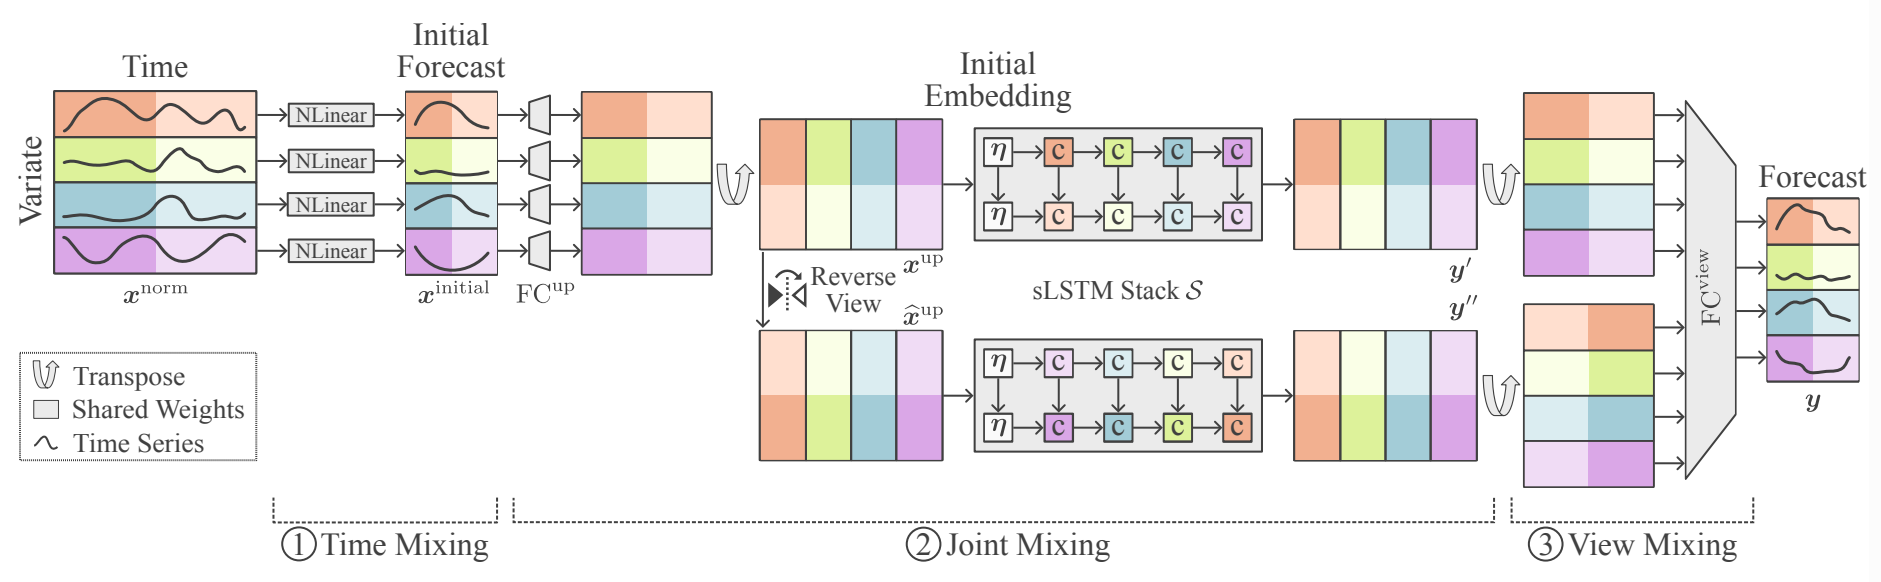
\includegraphics[width=0.95\linewidth]{../transformixer_paper/figures/xlstm-mixer-architecture.png}

  \vspace{0.4em}
  {\footnotesize Same temporal pipeline (RevIN + NLinear); Transformixer replaces joint/view mixing with a PE-free Transformer.}
\end{frame}

%---------------------------------------------------------------------
\begin{frame}{Idea: Transformixer}
  \textbf{Keep} what works: RevIN + shared NLinear temporal mixing.\\
  \textbf{Replace} the ordered sLSTM mixer with a PE-free Transformer over variate tokens.

  \vspace{0.8em}
  \centering
  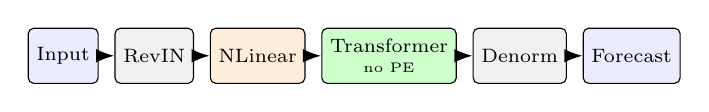
\begin{tikzpicture}[
    font=\scriptsize,
    box/.style={draw, rounded corners=2pt, align=center, inner sep=3pt, minimum height=7mm},
    arrow/.style={-{Latex}, thick}
  ]
    \node[box, fill=blue!8] (in) {Input};
    \node[box, fill=gray!12, right=0.2cm of in] (revin) {RevIN};
    \node[box, fill=orange!15, right=0.2cm of revin] (nlin) {NLinear};
    \node[box, fill=green!20, right=0.2cm of nlin] (tr) {Transformer\\[-1pt]{\tiny no PE}};
    \node[box, fill=gray!12, right=0.2cm of tr] (den) {Denorm};
    \node[box, fill=blue!8, right=0.2cm of den] (out) {Forecast};
    \foreach \a/\b in {in/revin,revin/nlin,nlin/tr,tr/den,den/out} \draw[arrow] (\a) -- (\b);
  \end{tikzpicture}

  \vspace{0.8em}
  \begin{itemize}
    \item Variates treated as a \textbf{set} (permutation-equivariant)
    \item Direct pairwise interactions via multi-head attention
    \item No memory tokens, no forward/reverse multi-view
  \end{itemize}
\end{frame}

%---------------------------------------------------------------------
\begin{frame}{vs.\ xLSTM-Mixer (what changes)}
  \centering
  \begin{tabular}{lcc}
    \toprule
    Component & xLSTM-Mixer & Transformixer \\
    \midrule
    RevIN + NLinear & yes & yes \\
    Variate mixer & sLSTM (+ mem.) & Transformer \\
    Positional bias on variates & via recurrence & \textbf{none} \\
    Forward/reverse views & yes & \textbf{no} \\
    Memory tokens & yes & \textbf{no} \\
    \bottomrule
  \end{tabular}

  \vspace{1em}
  \begin{block}{Related but different from iTransformer}
    iTransformer = full inverted backbone.\\
    Transformixer = attention as a \emph{drop-in mixer block} after NLinear.
  \end{block}
\end{frame}

%---------------------------------------------------------------------
\begin{frame}{Why Transformer mixing? (not only equivariance)}
  \begin{enumerate}
    \item \textbf{Direct global interactions} --- $O(1)$ path length between any pair of variates\\
    {\small (sLSTM propagates sequentially along an arbitrary order)}
    \item \textbf{Multi-head specialization} --- different dependency patterns in parallel
    \item \textbf{Simpler architecture} --- drop multi-view + memory tokens
    \item \textbf{Hardware-parallel over $C$} --- we measure training it/s; $O(C^2)$ caveat remains
  \end{enumerate}

  \vspace{0.6em}
  Hypothesis: PE-free attention should help most when $C$ is large (Traffic); PE is a separate, dataset-dependent knob.
\end{frame}

%---------------------------------------------------------------------
\begin{frame}{Experimental setup}
  \begin{columns}[T]
    \begin{column}{0.48\textwidth}
      \textbf{Datasets}: ECL ($C{=}321$), Traffic ($C{=}862$)\\
      \textbf{Protocol}: $L{=}H{=}96$; MSE/MAE; multivariate
      \vspace{0.4em}

      \textbf{Baselines}: RLinear, Informer, PatchTST, iTransformer, xLSTM-Mixer\\
      \textbf{Fairness}: baselines author-tuned; Transformixer not independently tuned
    \end{column}
    \begin{column}{0.48\textwidth}
      \textbf{Controlled ablation (same recipe)}\\
      A: NLinear only \quad B: xLSTM FULL\\
      C: Transformixer (no PE, default)\\
      D: Transformixer (+ PE)
      \vspace{0.4em}

      \begin{alertblock}{Scope}
        2 datasets, 1 horizon, single runs. Main table includes both Transformixer variants (C and D).
      \end{alertblock}
    \end{column}
  \end{columns}
\end{frame}

%---------------------------------------------------------------------
\begin{frame}{Main results}
  \centering
  {\scriptsize
  \begin{tabular}{lcccc}
    \toprule
    & \multicolumn{2}{c}{ECL} & \multicolumn{2}{c}{Traffic} \\
    \cmidrule(lr){2-3}\cmidrule(lr){4-5}
    Model & MSE & MAE & MSE & MAE \\
    \midrule
    RLinear      & 0.1973 & 0.2740 & 0.6463 & 0.3844 \\
    Informer     & 0.3263 & 0.4068 & 1.0140 & 0.5624 \\
    PatchTST     & 0.1754 & 0.2603 & 0.4699 & 0.3005 \\
    iTransformer & 0.1481 & 0.2398 & \textbf{0.3931} & 0.2687 \\
    xLSTM-Mixer  & \underline{0.1480} & \underline{0.2352} & 0.4157 & \underline{0.2607} \\
    Transformixer & 0.1517 & 0.2364 & \underline{0.4068} & \textbf{0.2558} \\
    Transformixer+PE & \textbf{0.1403} & \textbf{0.2315} & 0.4152 & 0.2639 \\
    \bottomrule
  \end{tabular}}

  \vspace{0.8em}
  \begin{itemize}
    \item \textbf{ECL:} Transformixer+PE best overall; PE-free default slightly behind xLSTM / iTransformer
    \item \textbf{Traffic:} PE-free default beats xLSTM-Mixer; \textbf{best MAE} overall; +PE slightly worse
    \item Positional bias is dataset-dependent (also confirmed in controlled ablation)
  \end{itemize}
\end{frame}

%---------------------------------------------------------------------
\begin{frame}{Results at a glance}
  \begin{columns}[c]
    \begin{column}{0.95\textwidth}
      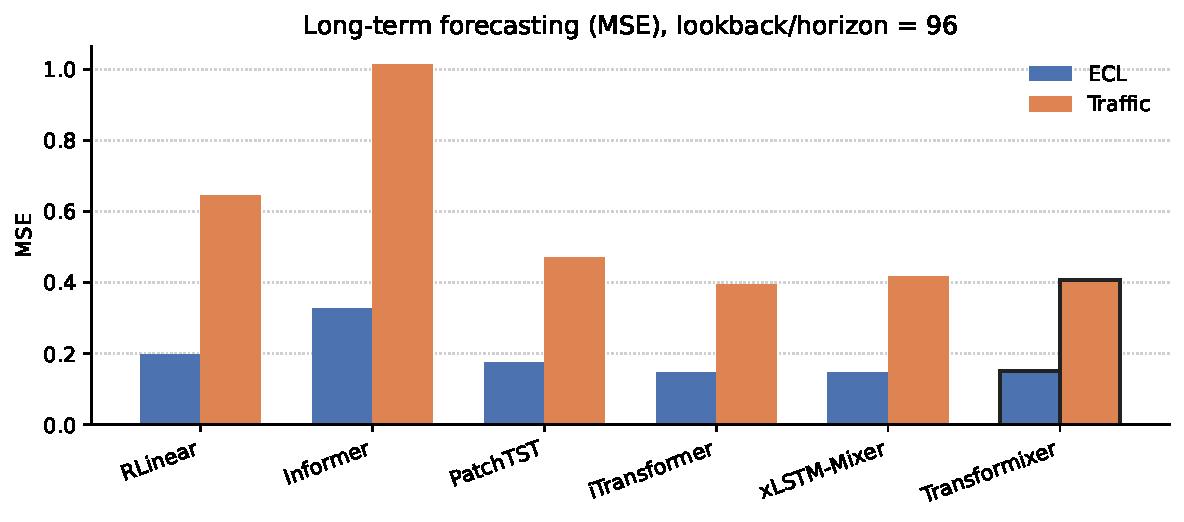
\includegraphics[width=\linewidth]{../transformixer_paper/figures/results_mse.pdf}
    \end{column}
  \end{columns}
  \vspace{0.3em}
  {\footnotesize Informer omitted for scale; y-axis zoomed around competitive models.}
\end{frame}

%---------------------------------------------------------------------
\begin{frame}{Mixer ablation (shared RevIN+NLinear)}
  \centering
  {\scriptsize
  \begin{tabular}{lcccc}
    \toprule
    & \multicolumn{2}{c}{ECL} & \multicolumn{2}{c}{Traffic} \\
    \cmidrule(lr){2-3}\cmidrule(lr){4-5}
    Variate mixer & MSE & MAE & MSE & MAE \\
    \midrule
    A: NLinear only          & 0.2016 & 0.2731 & 0.6713 & 0.3776 \\
    B: xLSTM FULL           & \underline{0.1480} & \underline{0.2352} & 0.4157 & \underline{0.2607} \\
    C: Transformixer (no PE) & 0.1517 & 0.2364 & \textbf{0.4068} & \textbf{0.2558} \\
    D: Transformixer (+ PE)  & \textbf{0.1403} & \textbf{0.2315} & \underline{0.4152} & 0.2639 \\
    \bottomrule
  \end{tabular}}

  \vspace{0.6em}
  \begin{itemize}
    \item Mixer $\gg$ NLinear-only on both datasets (esp.\ Traffic)
    \item \textbf{Traffic:} PE-free (C) best; fixed PE (D) hurts
    \item \textbf{ECL:} fixed PE (D) best; index-aware bias can help
  \end{itemize}
\end{frame}

%---------------------------------------------------------------------
\begin{frame}{Ablation at a glance}
  \centering
  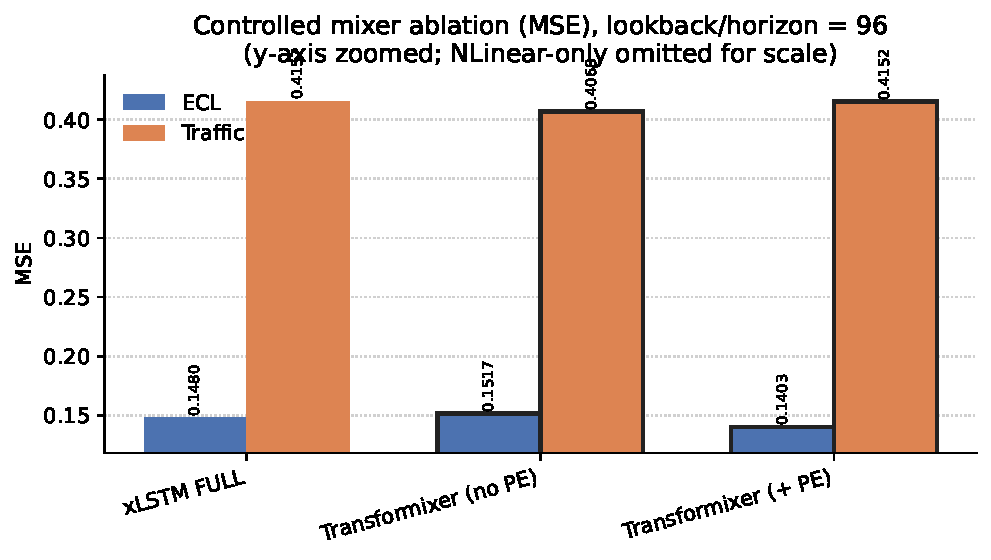
\includegraphics[width=0.92\linewidth]{../transformixer_paper/figures/ablation_mse.pdf}
  \vspace{0.3em}
  {\footnotesize NLinear-only omitted for scale; y-axis zoomed around mixer variants.}
\end{frame}

%---------------------------------------------------------------------
\begin{frame}{Permutation probe (Traffic checkpoints)}
  \centering
  {\small
  \begin{tabular}{lcccc}
    \toprule
    & \multicolumn{2}{c}{Identity} & \multicolumn{2}{c}{Over 9 orders (mean$\pm$std)} \\
    \cmidrule(lr){2-3}\cmidrule(lr){4-5}
    Model & MSE & MAE & MSE & MAE \\
    \midrule
    xLSTM-Mixer   & 1.3463 & 0.9224 & $1.3486{\pm}0.0015$ & $0.9233{\pm}0.0005$ \\
    Transformixer & 1.2841 & 0.9019 & $1.2865{\pm}0.0014$ & $0.9027{\pm}0.0005$ \\
    \bottomrule
  \end{tabular}}

  \vspace{0.8em}
  \begin{itemize}
    \item PE-free checkpoint: nearly invariant (equivariance)
    \item xLSTM mild drift (multi-view helps), but \textbf{always worse}
    \item Relative gap $\approx$ 4.6\% MSE / 2.2\% MAE on this probe
  \end{itemize}
\end{frame}

%---------------------------------------------------------------------
\begin{frame}{Attention visualization}
  \begin{columns}[c]
    \begin{column}{0.48\textwidth}
      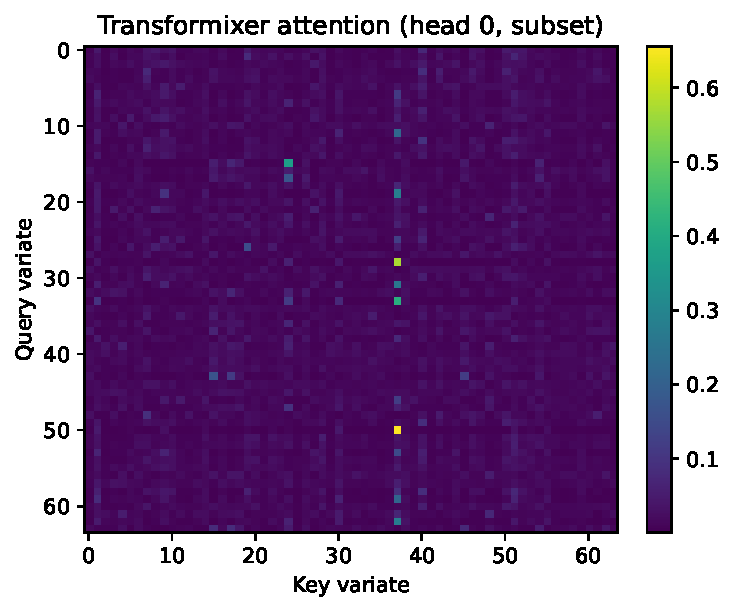
\includegraphics[width=\linewidth]{../transformixer_paper/figures/attention_heatmap.pdf}
    \end{column}
    \begin{column}{0.48\textwidth}
      \textbf{What we see}
      \begin{itemize}
        \item Sparse, non-uniform attention
        \item Hub-like key variates
        \item Not purely diagonal
      \end{itemize}
      \vspace{0.6em}
      Supports \emph{direct pairwise} cross-variate mixing.
    \end{column}
  \end{columns}
\end{frame}

%---------------------------------------------------------------------
\begin{frame}{Training throughput (NVIDIA L4)}
  \centering
  {\small
  \begin{tabular}{lccc}
    \toprule
    Dataset & $C$ & xLSTM-Mixer & Transformixer \\
    \midrule
    ECL     & 321 & 3.53 it/s & \textbf{4.67 it/s} \\
    Traffic & 862 & 1.32 it/s & 1.33 it/s \\
    \bottomrule
  \end{tabular}}

  \vspace{0.8em}
  \begin{itemize}
    \item \textbf{ECL:} Transformixer $\approx$32\% higher training throughput
    \item \textbf{Traffic:} essentially tied --- quadratic attention cost catches up at high $C$
    \item Progress-bar it/s (fwd+bwd, data loading, logging); \alert{not} FLOPs or inference latency
    \item No general wall-clock superiority claim
  \end{itemize}
\end{frame}

%---------------------------------------------------------------------
\begin{frame}{Limitations (stated openly)}
  \begin{itemize}
    \item Only \textbf{2 datasets}, horizon \textbf{96}, \textbf{single} runs
    \item Main baselines use author-tuned hparams; Transformixer not independently tuned
    \item Throughput is single-run it/s on L4; FLOPs / peak memory / inference not profiled
  \end{itemize}

  \vspace{0.6em}
  \begin{block}{Still useful}
    Main results and ablation agree: mixer is necessary; PE vs equivariance is dataset-dependent.\\
    Future work: learnable global permutations (e.g., Gumbel-Sinkhorn).
  \end{block}
\end{frame}

%---------------------------------------------------------------------
\begin{frame}{Takeaways}
  \begin{enumerate}
    \item \textbf{Transformixer} = NLinear temporal mix + PE-free Transformer variate mixer (default)
    \item Main results: +PE best on ECL; PE-free best Traffic MAE; bias is dataset-dependent
    \item Controlled ablation: mixer necessary; same PE vs equivariance pattern
    \item Throughput on L4: faster on ECL, tied on Traffic (parallelism vs $O(C^2)$)
    \item Future: learnable channel orderings via differentiable relaxations
  \end{enumerate}

  \vspace{1.2em}
  \centering
  {\Large Thank you}\\[0.6em]
  {\small Questions?}
\end{frame}

\end{document}
